\chapter{Societal Implications of Post-Quantum Cryptography}\label{chap:societal}

\section{Economic Impact}\label{sec:economic}

The transition to post-quantum cryptography will have significant economic implications:

\begin{itemize}
    \item \textbf{Infrastructure Costs:}
    \begin{itemize}
        \item Hardware upgrades
        \item Software modifications
        \item Training and implementation
    \end{itemize}
    \item \textbf{Market Opportunities:}
    \begin{itemize}
        \item New security products
        \item Consulting services
        \item Implementation expertise
    \end{itemize}
\end{itemize}

\section{Privacy and Security}\label{sec:privacy}

Long-term implications for privacy and security:

\begin{itemize}
    \item \textbf{Data Protection:}
    \begin{itemize}
        \item Historical data vulnerability
        \item Future privacy guarantees
        \item Regulatory compliance
    \end{itemize}
    \item \textbf{National Security:}
    \begin{itemize}
        \item Military communications
        \item Intelligence gathering
        \item Critical infrastructure
    \end{itemize}
\end{itemize}

\section{Digital Trust}\label{sec:trust}

Impact on trust in digital systems:

\begin{itemize}
    \item \textbf{Public Confidence:}
    \begin{itemize}
        \item Understanding of risks
        \item Trust in institutions
        \item Adoption of new systems
    \end{itemize}
    \item \textbf{Business Relations:}
    \begin{itemize}
        \item Supply chain security
        \item International trade
        \item Financial transactions
    \end{itemize}
\end{itemize}

\section{Policy Implications}\label{sec:policy}

Policy considerations for the post-quantum era:

\begin{itemize}
    \item \textbf{Regulation:}
    \begin{itemize}
        \item Compliance requirements
        \item International standards
        \item Export controls
    \end{itemize}
    \item \textbf{Government Action:}
    \begin{itemize}
        \item Research funding
        \item Infrastructure updates
        \item Public awareness
    \end{itemize}
\end{itemize}

\section{Educational Challenges}\label{sec:education}

Preparing for the post-quantum transition:

\begin{itemize}
    \item \textbf{Workforce Development:}
    \begin{itemize}
        \item Technical training
        \item Academic programs
        \item Professional certification
    \end{itemize}
    \item \textbf{Public Understanding:}
    \begin{itemize}
        \item Risk awareness
        \item Security practices
        \item Technology literacy
    \end{itemize}
\end{itemize}

\section{Global Impact}\label{sec:global}

International implications and considerations:

\begin{itemize}
    \item \textbf{Digital Divide:}
    \begin{itemize}
        \item Access to technology
        \item Implementation capacity
        \item Resource distribution
    \end{itemize}
    \item \textbf{International Cooperation:}
    \begin{itemize}
        \item Standards development
        \item Information sharing
        \item Joint research
    \end{itemize}
\end{itemize}

\section{Future Considerations}\label{sec:future}

Long-term societal considerations:

\begin{itemize}
    \item \textbf{Technological Evolution:}
    \begin{itemize}
        \item Ongoing innovation
        \item Adaptation requirements
        \item Future threats
    \end{itemize}
    \item \textbf{Social Adaptation:}
    \begin{itemize}
        \item Cultural changes
        \item Behavioral adjustments
        \item Risk perception
    \end{itemize}
\end{itemize}

\section{Recommendations}\label{sec:recommendations}

Policy and action recommendations:

\begin{enumerate}
    \item Develop comprehensive transition strategies
    \item Establish international cooperation frameworks
    \item Create public awareness programs
    \item Invest in education and training
    \item Support ongoing research and development
    \item Implement regular assessment mechanisms
\end{enumerate}

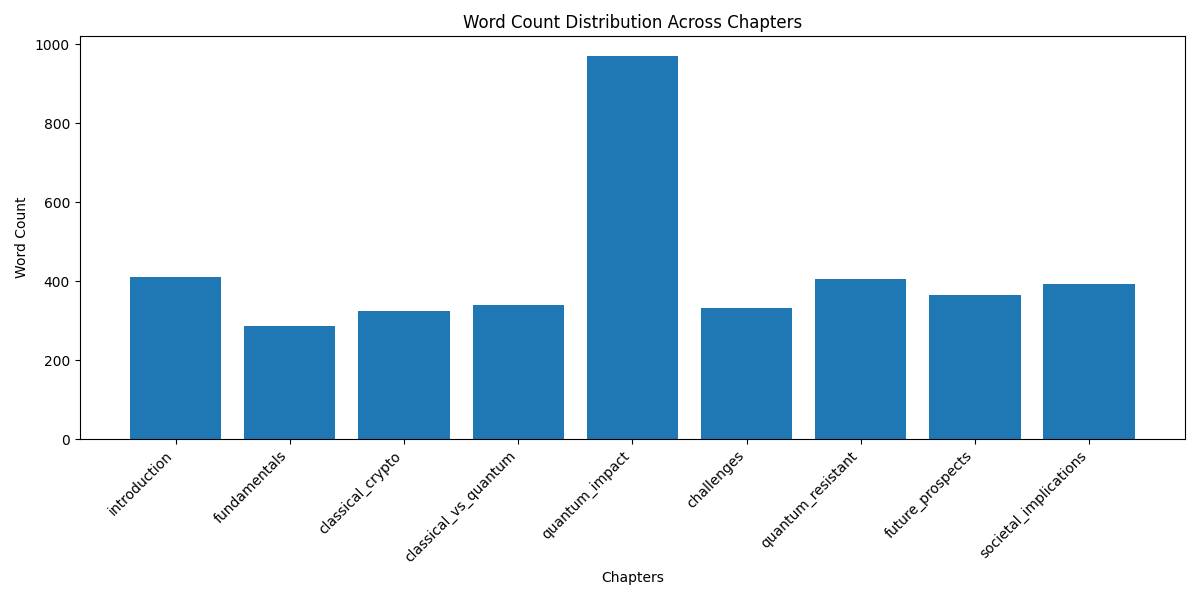
\includegraphics[width=0.8\textwidth]{09_Societal_Implications/word_distribution}

The societal implications of post-quantum cryptography extend far beyond technical considerations, requiring careful attention to economic, social, and policy dimensions to ensure a successful transition to quantum-resistant security systems.